\documentclass[]{article}


%-----------------------------------------------------------------------------------------------------------------------------------------
%
%   GLOBALS
%
%-----------------------------------------------------------------------------------------------------------------------------------------
\newcommand{\DOCTITLE}{

}
\newcommand{\DOCAUTHOR}{

}
\newcommand{\DISCLAIMER}
{
    \topskip0pt
    \vspace*{\fill}
    {
    \centering
        \small{
            THIS DOCUMENT IS INTENDED FOR INTERNAL USE ONLY
        }
    }
    \\
    {
    \centering
        \small{
        UNAUTHORIZED DISTRIBUTION OF THIS DOCUMENT IS STRICTLY PROHIBITED 
        }
    }
    \vspace*{\fill}
}

\usepackage{lmodern}
\usepackage{amssymb,amsmath}
\usepackage{ifxetex,ifluatex}
\usepackage{fixltx2e} % provides \textsubscript
\ifnum 0\ifxetex 1\fi\ifluatex 1\fi=0 % if pdftex
  \usepackage[T1]{fontenc}
  \usepackage[utf8]{inputenc}
\else % if luatex or xelatex
  \ifxetex
    \usepackage{mathspec}
    \usepackage{xltxtra,xunicode}
  \else
    \usepackage{fontspec}
  \fi
  \defaultfontfeatures{Mapping=tex-text,Scale=MatchLowercase}
  \newcommand{\euro}{€}
\fi
% use upquote if available, for straight quotes in verbatim environments
\IfFileExists{upquote.sty}{\usepackage{upquote}}{}
% use microtype if available
\IfFileExists{microtype.sty}{%
\usepackage{microtype}
\UseMicrotypeSet[protrusion]{basicmath} % disable protrusion for tt fonts
}{}
\ifxetex
  \usepackage[setpagesize=false, % page size defined by xetex
              unicode=false, % unicode breaks when used with xetex
              xetex]{hyperref}
\else
  \usepackage[unicode=true]{hyperref}
\fi
\usepackage[usenames,dvipsnames]{color}
\hypersetup{breaklinks=true,
            bookmarks=true,
            pdfauthor={},
            pdftitle={},
            colorlinks=true,
            citecolor=blue,
            urlcolor=blue,
            linkcolor=magenta,
            pdfborder={0 0 0}}
\urlstyle{same}  % don't use monospace font for urls
\usepackage{longtable,booktabs}
\usepackage{graphicx,grffile}
\makeatletter
\def\maxwidth{\ifdim\Gin@nat@width>\linewidth\linewidth\else\Gin@nat@width\fi}
\def\maxheight{\ifdim\Gin@nat@height>\textheight\textheight\else\Gin@nat@height\fi}
\makeatother
% Scale images if necessary, so that they will not overflow the page
% margins by default, and it is still possible to overwrite the defaults
% using explicit options in \includegraphics[width, height, ...]{}
\setkeys{Gin}{width=\maxwidth,height=\maxheight,keepaspectratio}
\setlength{\parindent}{0pt}
\setlength{\parskip}{6pt plus 2pt minus 1pt}
\setlength{\emergencystretch}{3em}  % prevent overfull lines
\providecommand{\tightlist}{%
  \setlength{\itemsep}{0pt}\setlength{\parskip}{0pt}}
\setcounter{secnumdepth}{0}

\date{}

% Redefines (sub)paragraphs to behave more like sections
\ifx\paragraph\undefined\else
\let\oldparagraph\paragraph
\renewcommand{\paragraph}[1]{\oldparagraph{#1}\mbox{}}
\fi
\ifx\subparagraph\undefined\else
\let\oldsubparagraph\subparagraph
\renewcommand{\subparagraph}[1]{\oldsubparagraph{#1}\mbox{}}
\fi

%-----------------------------------------------------------------------------------------------------------------------------------------
%
%   PAGE SIZE AND MARGINS
%
%-----------------------------------------------------------------------------------------------------------------------------------------
\usepackage[a4paper,headheight=30pt]{geometry}
%\usepackage[letterpaper, portrait, margin=2in]{geometry}
\addtolength{\topmargin}{-.5in}
\addtolength{\textheight}{1.75in}

\usepackage{graphicx}

\usepackage{fancyhdr}
\pagestyle{fancy}


%-----------------------------------------------------------------------------------------------------------------------------------------
% Page break after sections
%-----------------------------------------------------------------------------------------------------------------------------------------
%\usepackage{titlesec}
%\newcommand{\sectionbreak}{\clearpage}

\lhead{
    %left header content
%    \topskip0pt
%    \vspace*{\fill}
    {
    \centering
        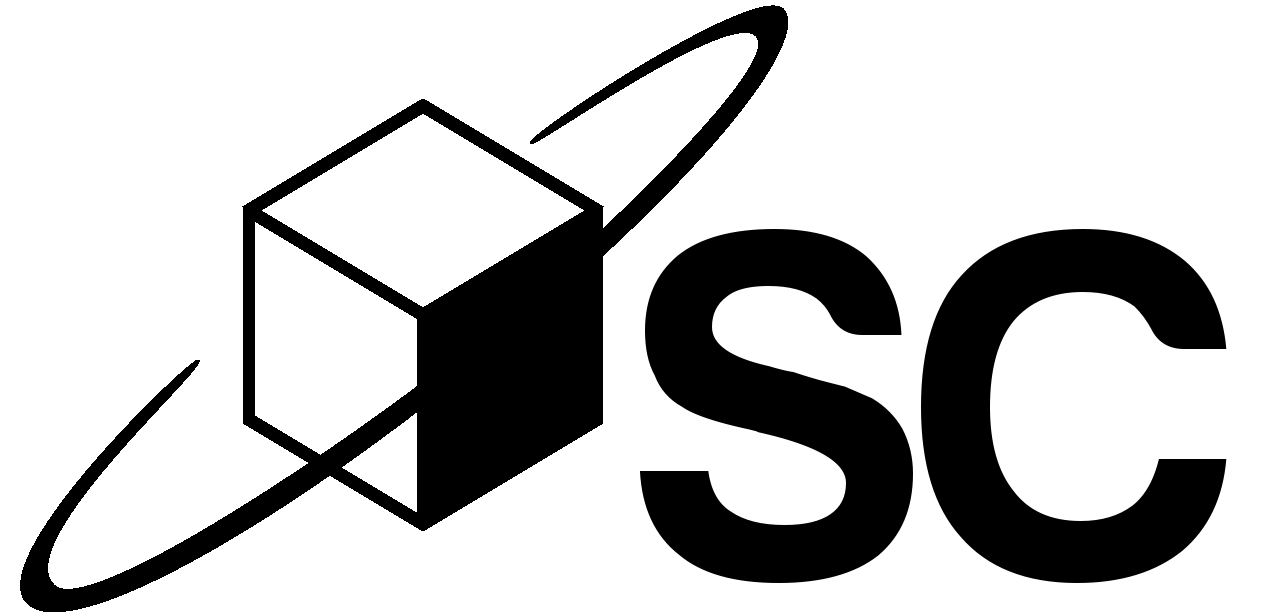
\includegraphics[height=2.66em]{template/sc.png}
    }
%    \vspace*{\fill}
}
\chead{
    \topskip0pt
    \vspace*{\fill}
    {
    \centering
        \small{
            THIS DOCUMENT IS INTENDED FOR INTERNAL USE ONLY
        }
    }
    \\
    {
    \centering
        \small{
        UNAUTHORIZED DISTRIBUTION OF THIS DOCUMENT IS STRICTLY PROHIBITED 
        }
    }
    \vspace*{\fill}
}
\rhead{
%    \topskip0pt
%    \vspace*{\fill}
    % right header content
    {
    \centering
        
\includegraphics[height=3.25em]{template/scrd.png}
    }
%    \vspace*{\fill}
}
\lfoot{
    % left footer content
    \topskip0pt
    \vspace*{\fill}
    SCRD
    Revision 0.1
    \vspace*{\fill}
}
\cfoot{
    % middle footer content
    \topskip0pt
    \vspace*{\fill}
    {
    \centering
    SCRD Internal Documents Template \\
    \today
    }
    \vspace*{\fill}
}
\rfoot{
    % right footer content
    \topskip0pt
    \vspace*{\fill}
    \thepage
    \vspace*{\fill}
}
% extend the header into the margins
\usepackage{calc}
\fancyheadoffset[L,R]{\marginparsep+\marginparwidth}

%--------------------------------------------------------------------------------------------------------------
%	My Packages
%--------------------------------------------------------------------------------------------------------------
\usepackage{capt-of}

%--------------------------------------------------------------------------------------------------------------
%
%	BEGIN DOCUMENT
%
%--------------------------------------------------------------------------------------------------------------
\begin{document}


%--------------------------------------------------------------------------------------------------------------
%
%	TITLE PAGE
%
%--------------------------------------------------------------------------------------------------------------
\begin{titlepage}

\newcommand{\HRule}{\rule{\linewidth}{0.5mm}} % Defines a new command for the horizontal lines, change thickness here

\center % Center everything on the page
 
%----------------------------------------------------------------------------------------
%	HEADING SECTIONS
%----------------------------------------------------------------------------------------

\includegraphics[width=200pt,height=200pt]{../images/rocketry_logo_large.png}\\[1cm] % Include a department/university logo - this will require the graphicx package
\textsc{\Large Space Concordia - Rocketry Division}\\[0.5cm] % Major heading such as course name
\textsc{\large Aurelius CR-2-4G - Structural Team}\\[0.5cm] % Minor heading such as course title

%----------------------------------------------------------------------------------------
%	LOGO SECTION
%----------------------------------------------------------------------------------------

\begin{figure}[ht]
    \centering
    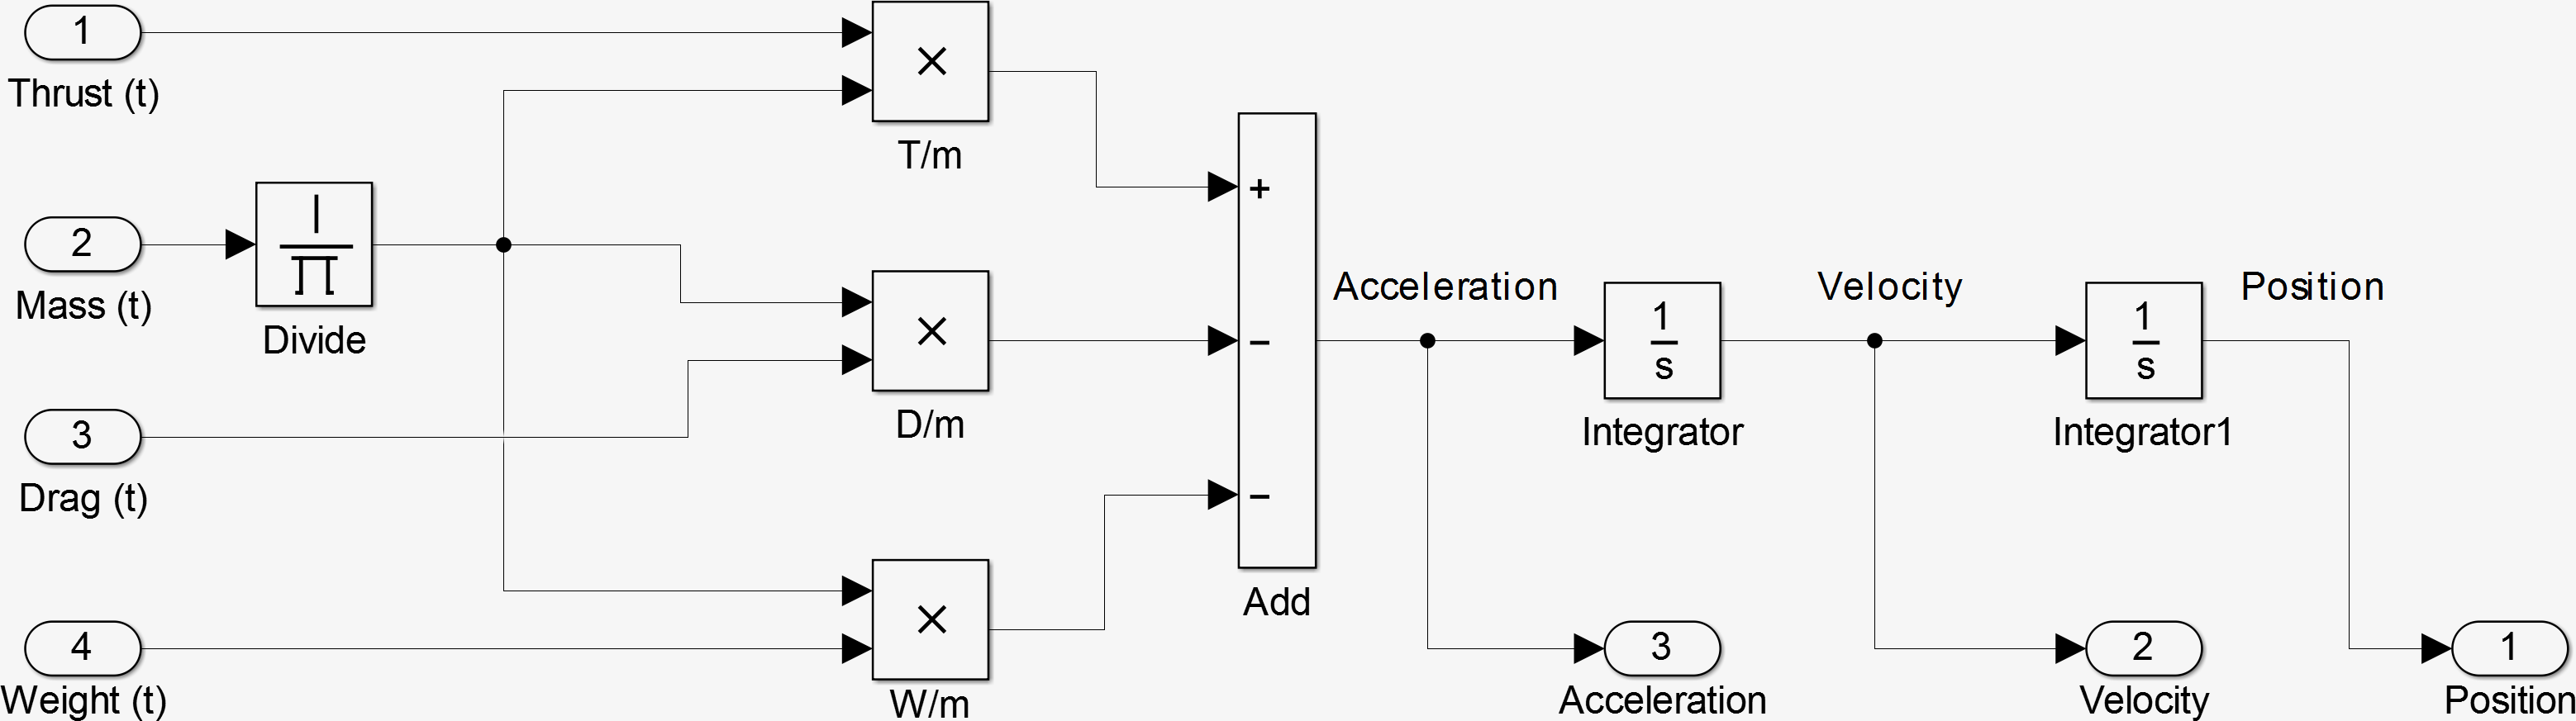
\includegraphics[height=100pt]{../images/vertical_model_simplified.png}\\
\end{figure}

%----------------------------------------------------------------------------------------
%	TITLE SECTION
%----------------------------------------------------------------------------------------

\HRule \\[0.6cm]
{ \Huge \bfseries 
Engineering Simulation for Rocket Flight Analysis
}\\[0.4cm] 

\HRule \\[1cm]
 
%----------------------------------------------------------------------------------------
%	AUTHOR SECTION
%----------------------------------------------------------------------------------------

\begin{minipage}{0.4\textwidth}
\begin{flushleft} \large
	\begin{tabular} {r l} 
        \emph{Author(s):} & Shawn Bulger	\\
	\end{tabular}
\end{flushleft}
\end{minipage}
~
\begin{minipage}{0.4\textwidth}
\begin{flushright} \large
	\begin{tabular} {r l} 
		\emph{Coordinator:} & Dr. Ashok Kaushal 		\\
		\emph{Supervisor:}  & Dr. Mehdi Hojjati 		\\
		\emph{EIR:}         & Dominic Ng  		        \\
	\end{tabular}
\end{flushright}
\end{minipage}\\[2cm]

%----------------------------------------------------------------------------------------
%	DATE SECTION
%----------------------------------------------------------------------------------------

{\large \today}\\[2cm] % Date, change the \today to a set date if you want to be precise

\vfill % Fill the rest of the page with whitespace

\end{titlepage}

{
\hypersetup{linkcolor=black}
\setcounter{tocdepth}{3}
\tableofcontents
\clearpage
}
\listoftables
\listoffigures
\clearpage
\section{Simulation Execution}\label{simulation-execution}

\subsection{Simulation Configuration}\label{simulation-configuration}

\subsubsection{Historical Weather Data for Green River,
Utah}\label{historical-weather-data-for-green-river-utah}

\begin{longtable}[c]{@{}llllll@{}}
\toprule
Date & Elevation & Ground Pressure & Ground Temperature & Wind Speed &
Humidity\tabularnewline
\midrule
\endhead
2015/06/15 & 4,078 ft (1,243 m) & 101300 Pa & 298.15 K (25 \(^\circ\)C)
& 6 km/h (1.6 m/s) & 33 \%\tabularnewline
2014/06/15 & 4,078 ft (1,243 m) & 100700 Pa & 296.15 K (23 \(^\circ\)C)
& 20 km/h (5.56 m/s) & 8 \%\tabularnewline
2013/06/15 & 4,078 ft (1,243 m) & 101000 Pa & 299.15 K (26 \(^\circ\)C)
& 10 km/h (2.78 m/s) & 19 \%\tabularnewline
\bottomrule
\end{longtable}

\captionof{table}{Historical Weather Conditions, Green River, Utah}

\subsubsection{General Conditions}\label{general-conditions}

For all tests, the following conditions were used, based on historical
data for June 25th, 2015 at 12:00PM (noon) near Green River, Utah
{[}1{]}.

\begin{longtable}[c]{@{}lll@{}}
\toprule
Elevation & Humidity & Launch Guide Length\tabularnewline
\midrule
\endhead
4,078 ft (1,243 m) {\textbf{???}} & 33 \% & 5.4864 (18
ft)\tabularnewline
\bottomrule
\end{longtable}

\captionof{table}{General Simulation Conditions}

\subsubsection{Best Case}\label{best-case}

The best case scenario is with no wind, and a 0\(^\circ\) launch angle,
and the lowest air pressure.

\begin{longtable}[c]{@{}llll@{}}
\toprule
Wind Speed & Ground Pressure & Ground Temperature & Launch Guide
Angle\tabularnewline
\midrule
\endhead
0 m/s & 101000 Pa & 298.15 K (25 \(^\circ\)C) &
0\(^\circ\)\tabularnewline
\bottomrule
\end{longtable}

\captionof{table}{Best Case Simulation Conditions}

\subsubsection{Worst Case}\label{worst-case}

The worst case scenario, is the maximum wind condition permitted for
launch by the competition, and a launch guide angle, and the highest
pressure.

\begin{longtable}[c]{@{}llll@{}}
\toprule
Wind Speed & Ground Pressure & Ground Temperature & Launch Guide
Angle\tabularnewline
\midrule
\endhead
8.33 m/s & 101325 kPa & 288.15 K (15 \(^\circ\)C) &
10\(^\circ\)\tabularnewline
\bottomrule
\end{longtable}

\captionof{table}{Worst Case Simulation Conditions}

\clearpage

\subsection{Simulation Software}\label{simulation-software}

The following models were executed.

\subsubsection{OpenRocket}\label{openrocket}

\subsubsection{RockSim}\label{rocksim}

\subsubsection{RASAero}\label{rasaero}

\clearpage

\subsubsection{Matlab}\label{matlab}

\paragraph{Matlab Models}\label{matlab-models}

\begin{figure}[htbp]
\centering
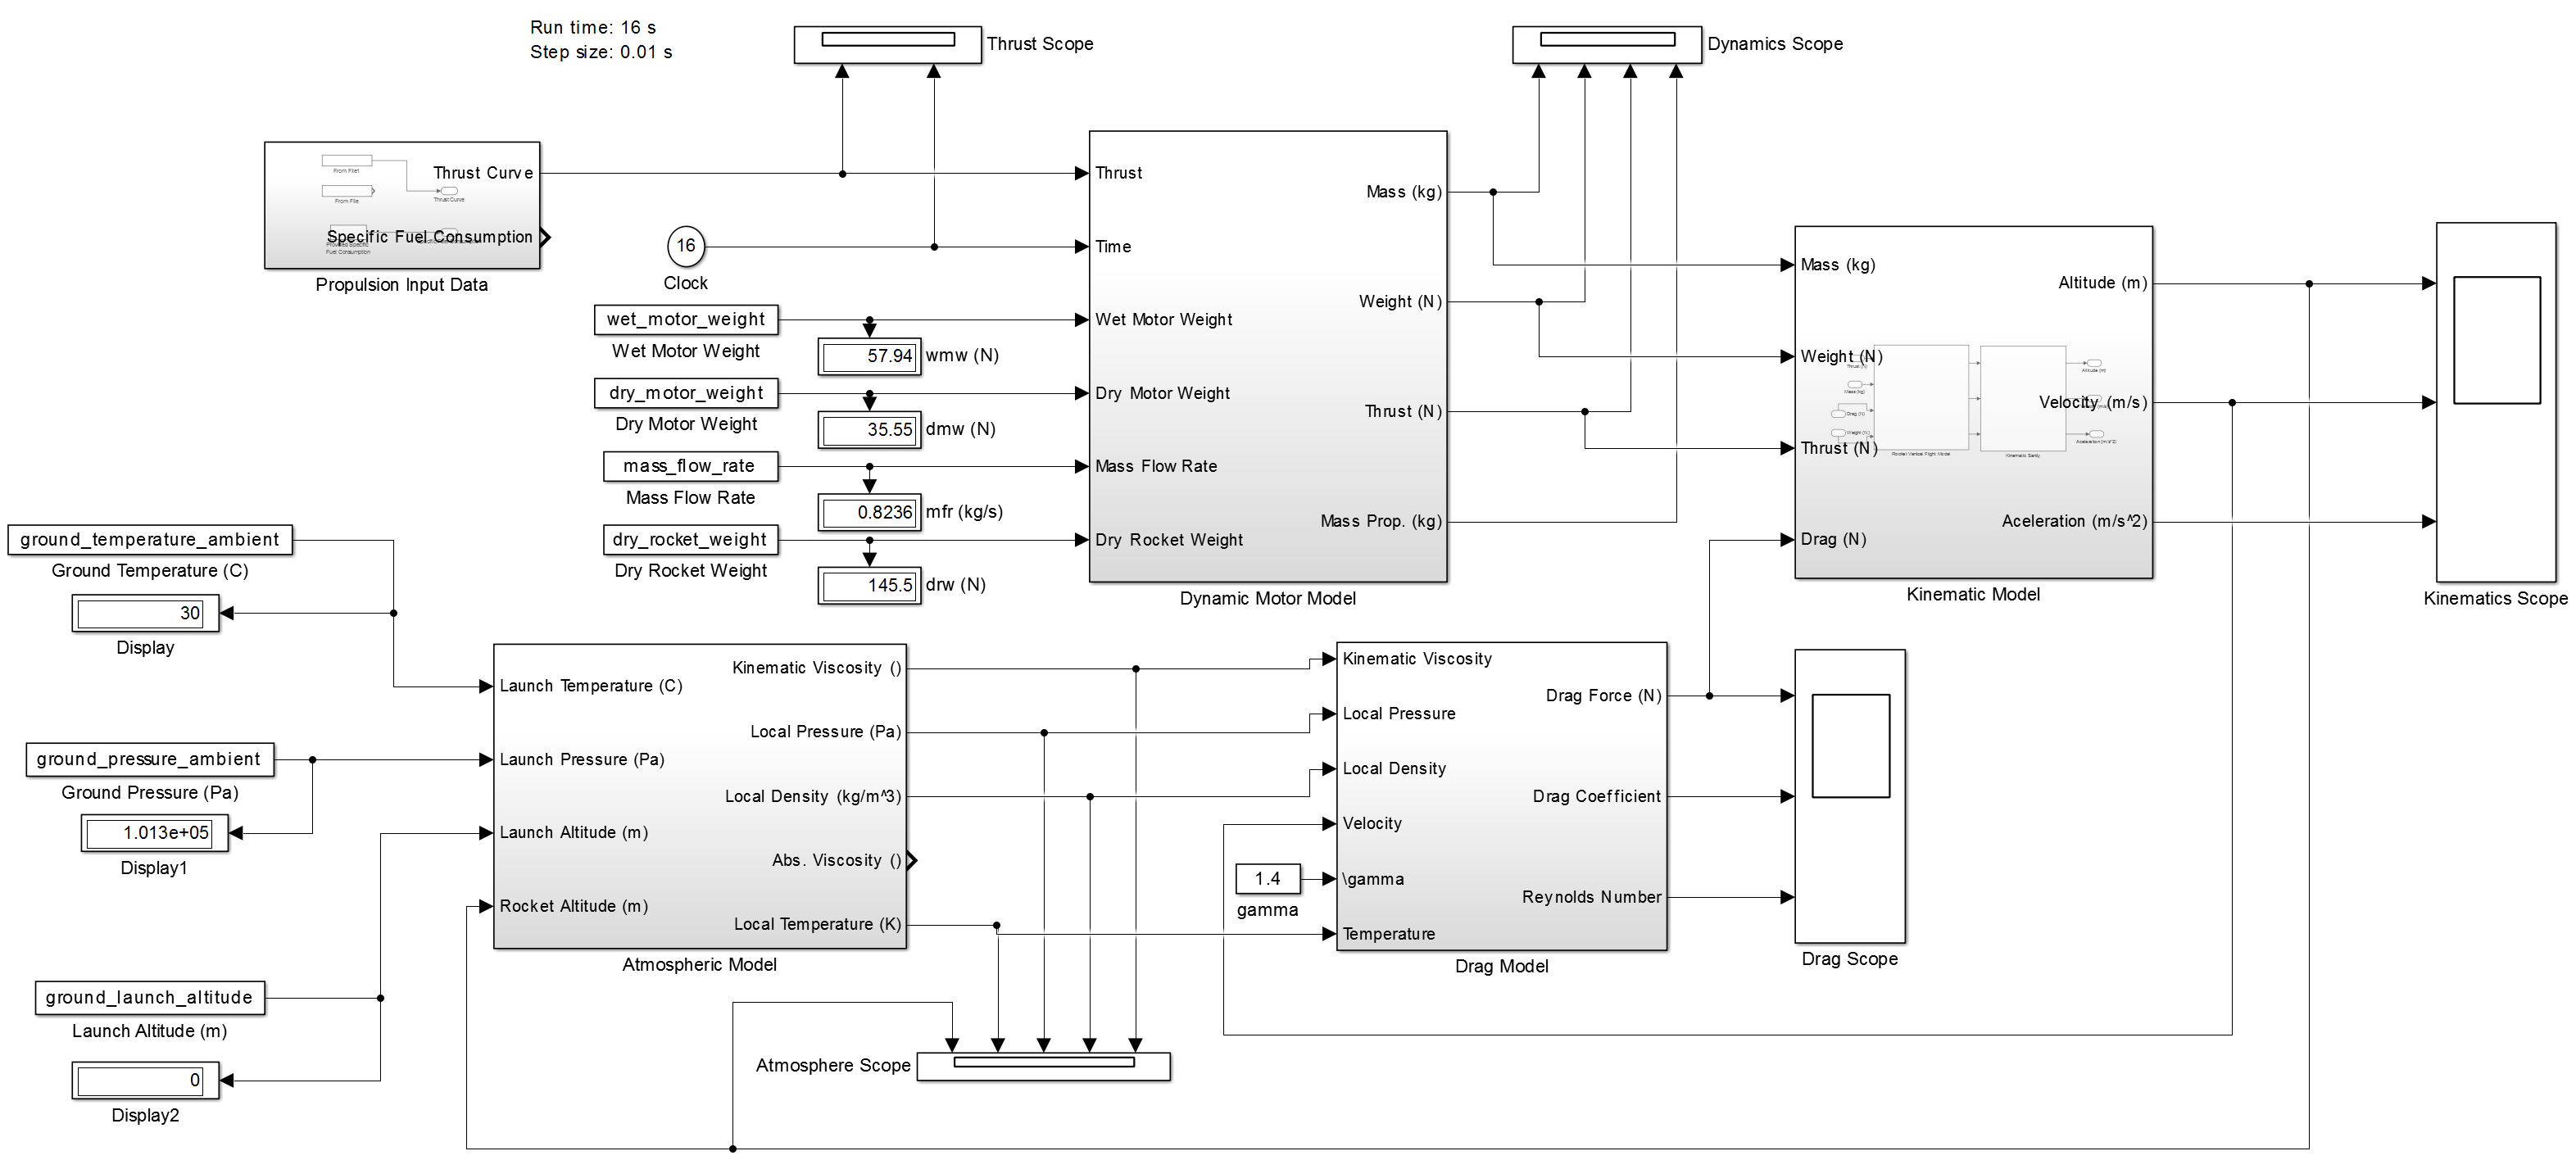
\includegraphics{images/vertical_model.png}
\caption{Vertical Model in Simulink, angle of attack less than 5 degrees
\label{vertical_model_test_label}}
\end{figure}

\begin{figure}[htbp]
\centering
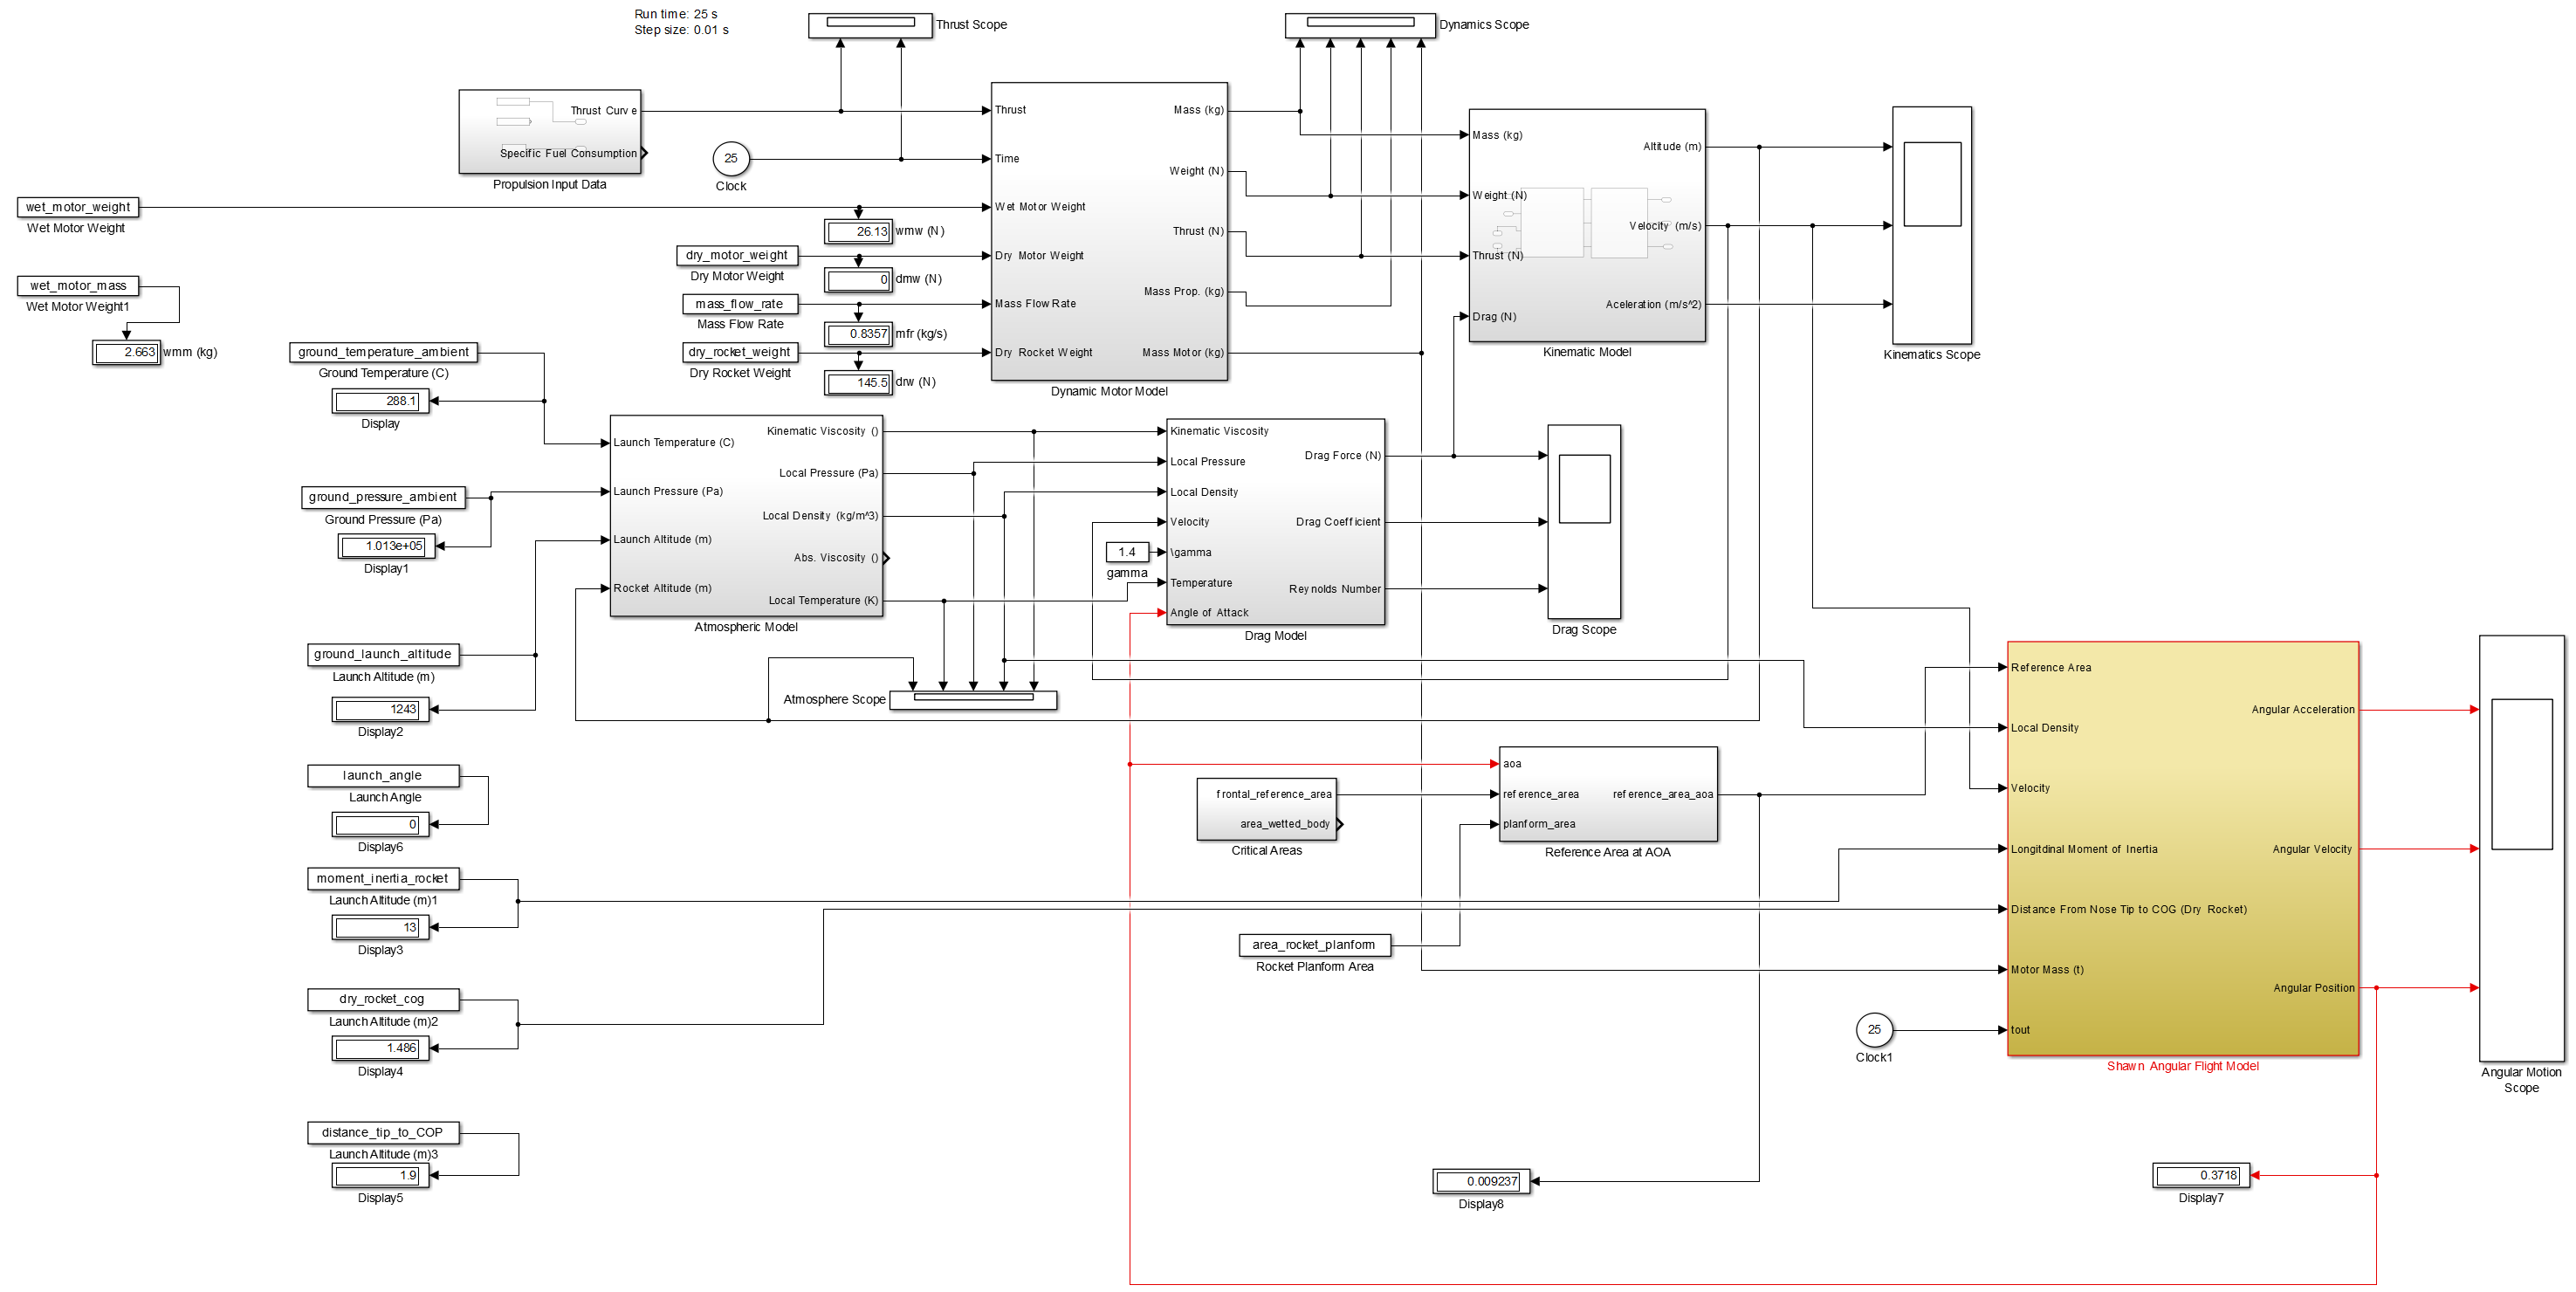
\includegraphics{images/rocket_model.png}
\caption{Full Model in Simulink, angle of attack less than 15 degrees
\label{full_model_test_label}}
\end{figure}

\clearpage

\subsection{Summary}\label{summary}

\subsubsection{Best Case}\label{best-case-1}

\begin{longtable}[c]{@{}lllllll@{}}
\toprule
Software & Case & Velocity leaving launch rail & Max Acc. & Max Vel. &
Max. Alt. & Time to apogee\tabularnewline
\midrule
\endhead
\bottomrule
\end{longtable}

\subsubsection{Worst Case}\label{worst-case-1}

\begin{longtable}[c]{@{}lllllll@{}}
\toprule
Software & Case & Velocity leaving launch rail & Max Acc. & Max Vel. &
Max. Alt. & Time to apogee\tabularnewline
\midrule
\endhead
\bottomrule
\end{longtable}

\subsection{Observations}\label{observations}

\clearpage

\subsection{Primary Plots}\label{primary-plots}

\begin{figure}[htbp]
\centering
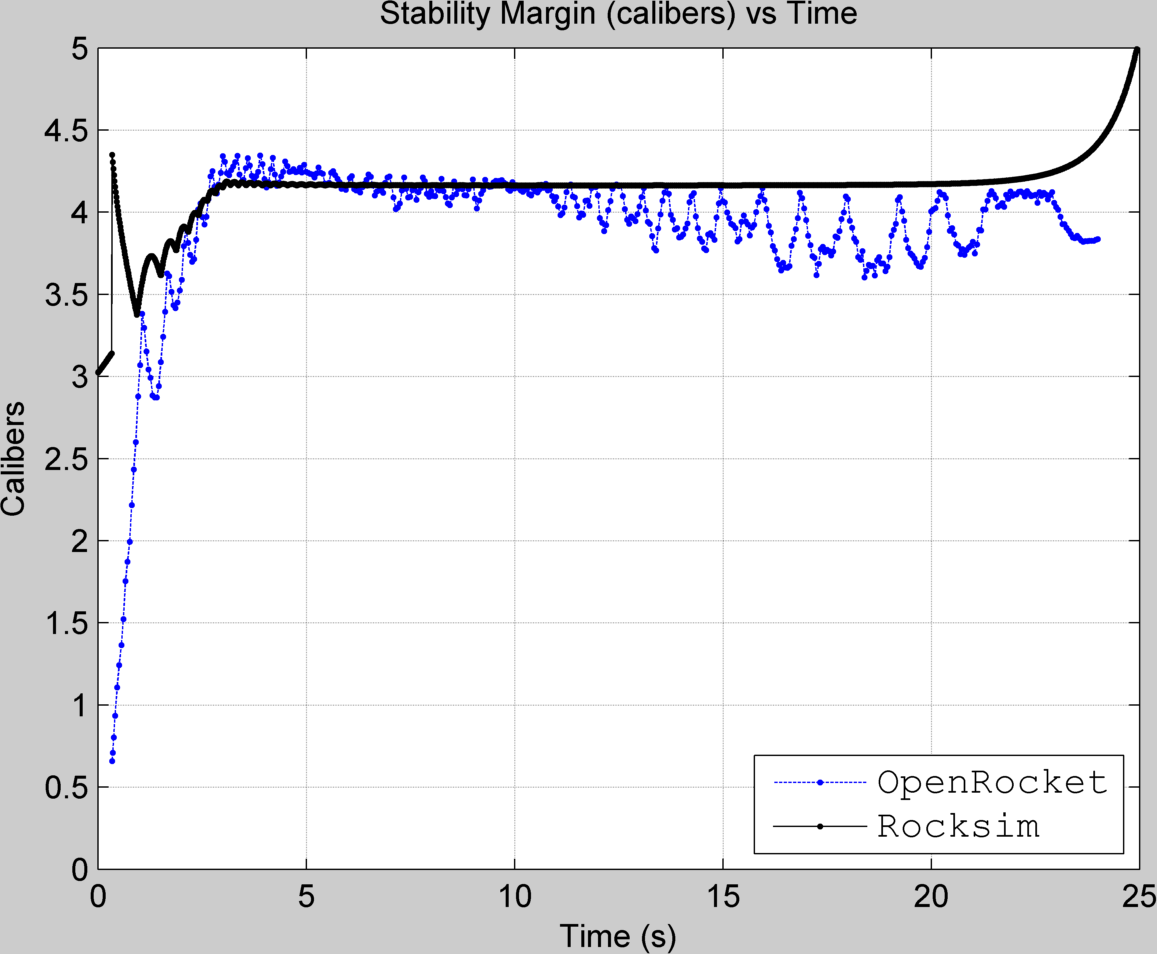
\includegraphics{images/plots/error_altitude_plot.png}
\caption{Altitude as a Function of Time
\label{error_altitude_plot_label}}
\end{figure}

\begin{figure}[htbp]
\centering
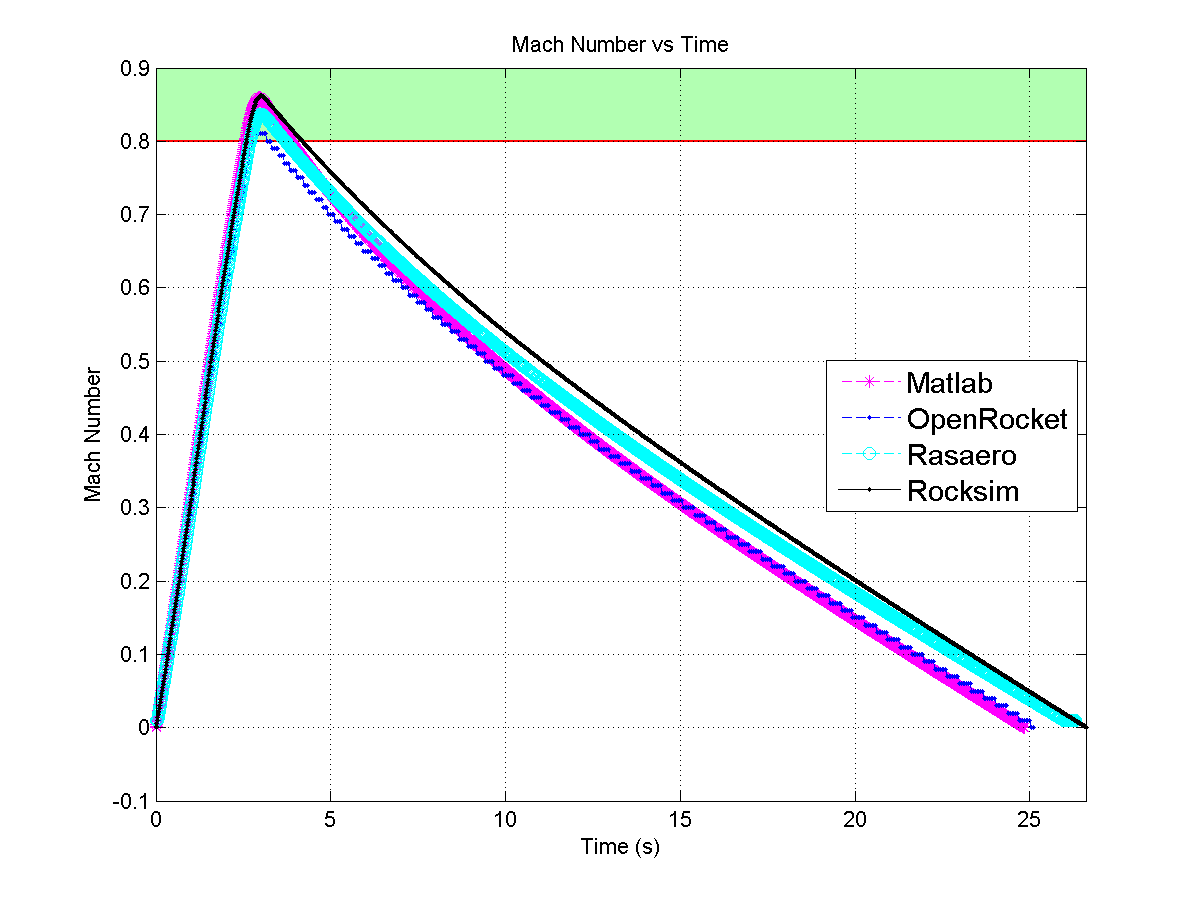
\includegraphics{images/plots/error_mach_plot.png}
\caption{Mach Number as a Function of Time
\label{error_mach_plot_label}}
\end{figure}

\begin{figure}[htbp]
\centering
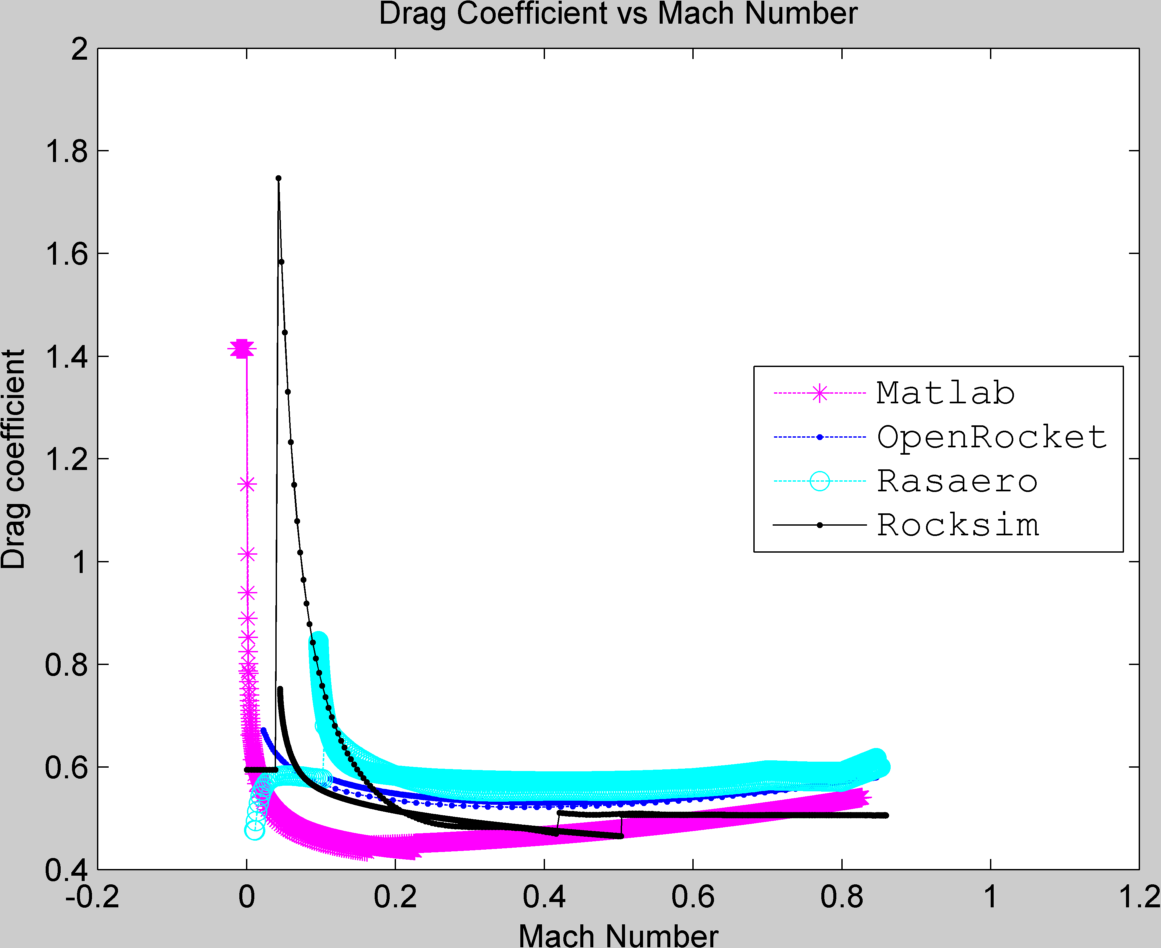
\includegraphics{images/plots/error_dragcoef_v_mach_plot.png}
\caption{Drag Coefficient as a Function of Mach Number
\label{error_dragcoef_v_plot_label}}
\end{figure}

\begin{figure}[htbp]
\centering
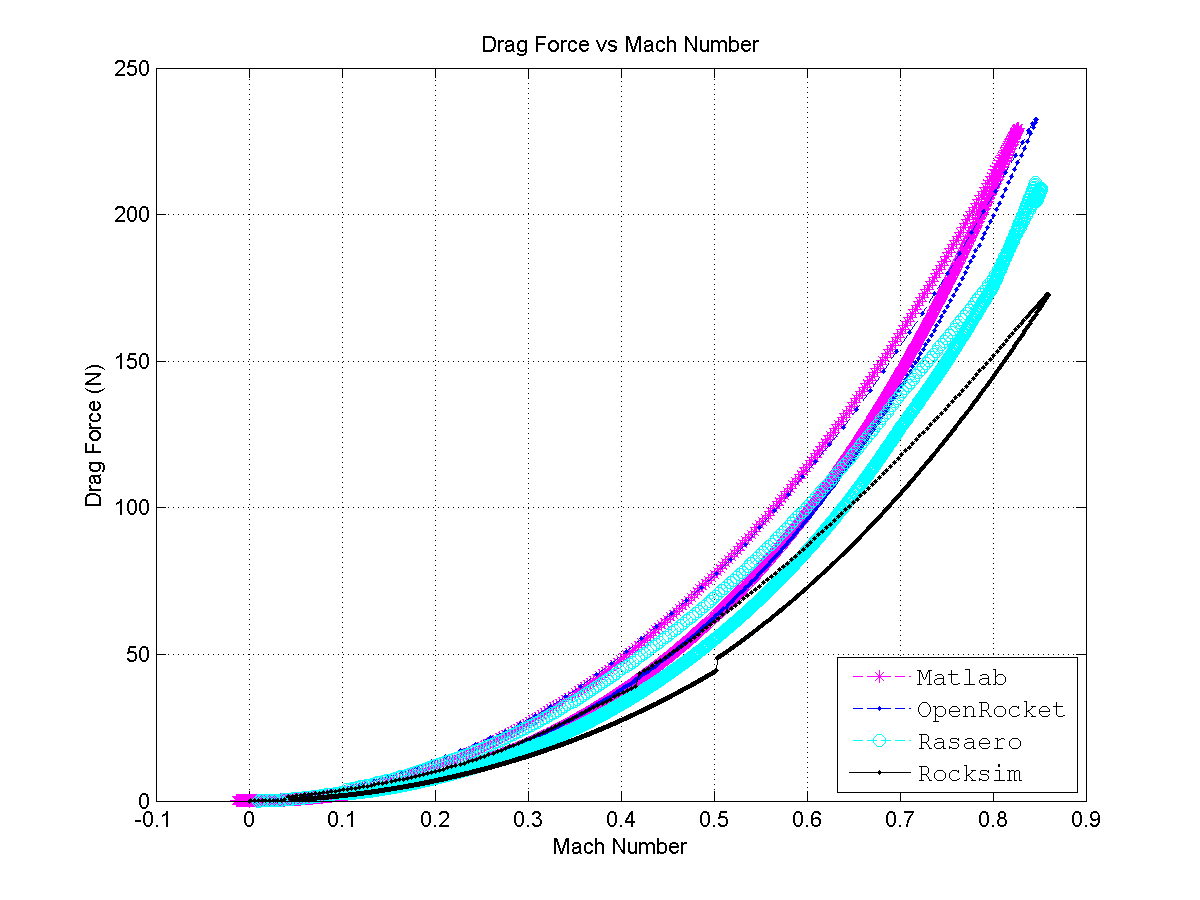
\includegraphics{images/plots/error_dragforce_plot.png}
\caption{Drag Force as a Function of Mach Number
\label{error_dragforce_v_plot_label}}
\end{figure}

\begin{figure}[htbp]
\centering
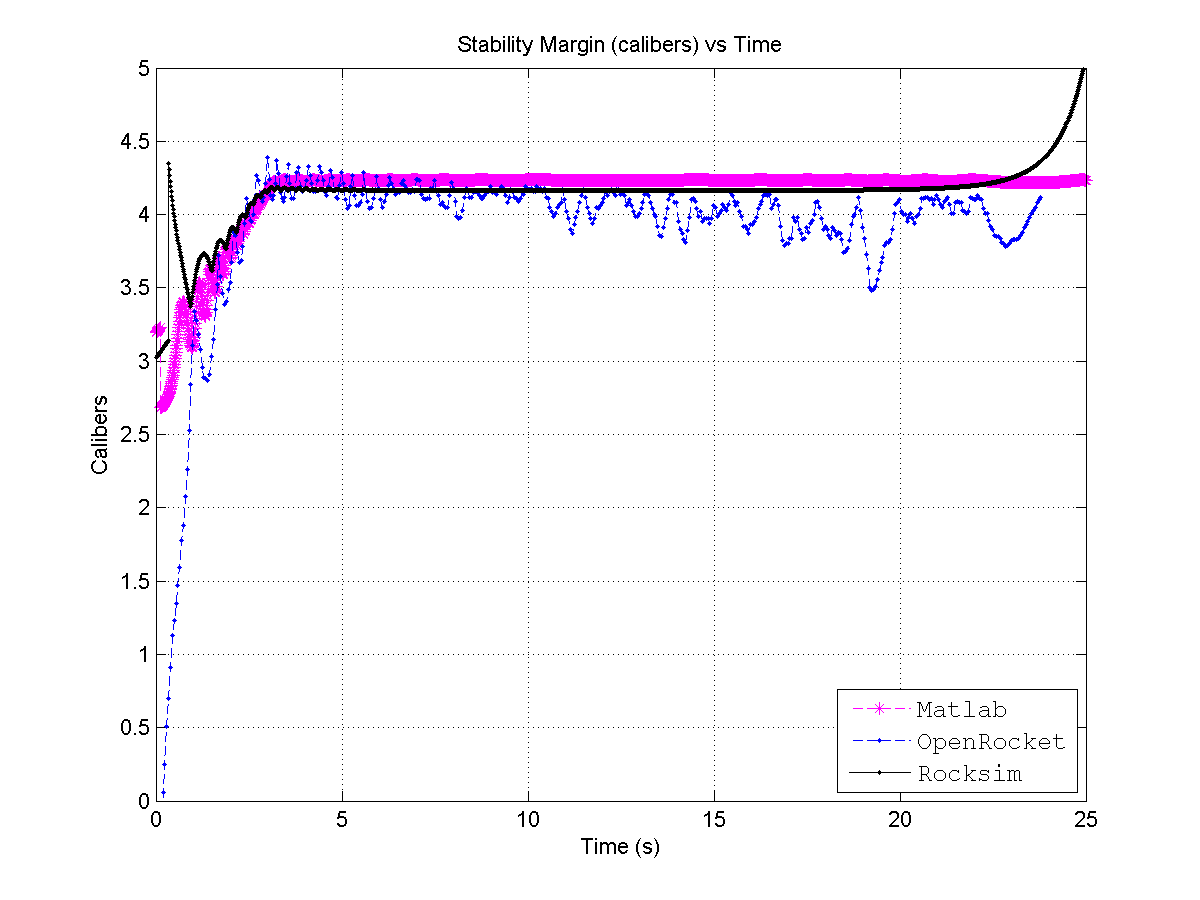
\includegraphics{images/plots/error_stability_calibers_plot.png}
\caption{Stability (Calibers) as a Function of Time
\label{error_stability_calibers_plot_label}}
\end{figure}

\begin{figure}[htbp]
\centering
\includegraphics{images/plots/plot_stability_response_homogeneous.png}
\caption{Homogeneous Response to Initial Conditions
\label{error_stability_response_homogeneous}}
\end{figure}

\clearpage

\subsubsection{Additional Plots}\label{additional-plots}

\begin{figure}[htbp]
\centering
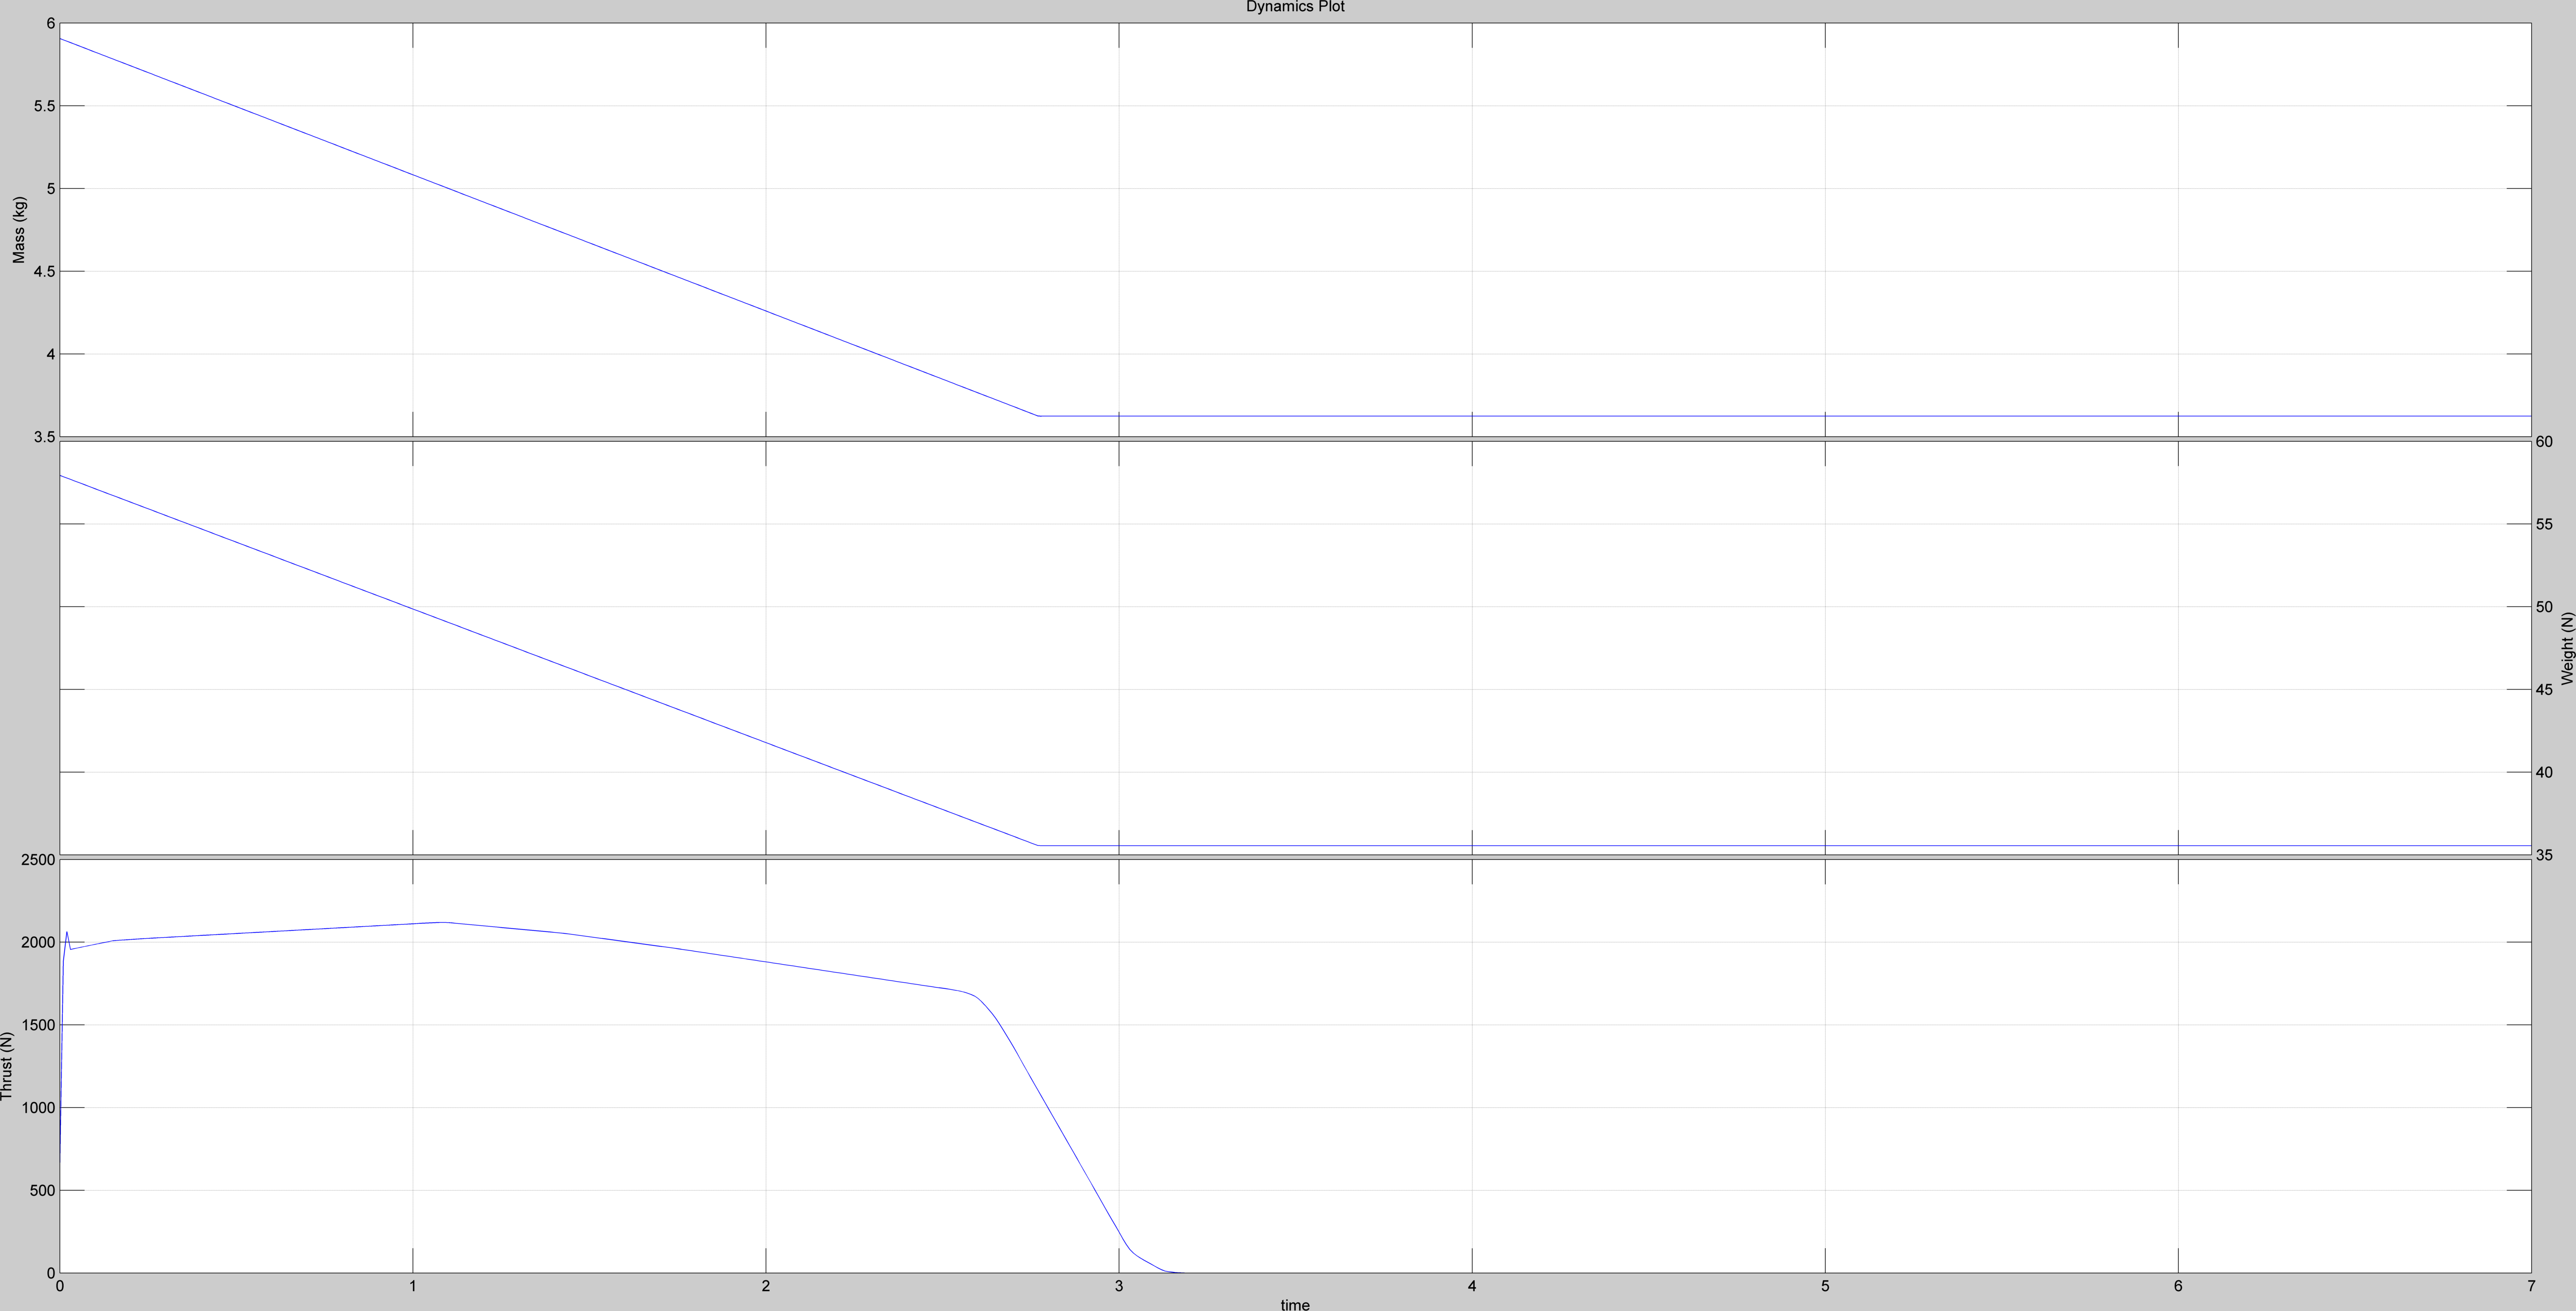
\includegraphics{images/plots/dynamics_plot.png}
\caption{Mass, Weight, and Thrust as a Function of Time
\label{dynamics_plot_label}}
\end{figure}

\begin{figure}[htbp]
\centering
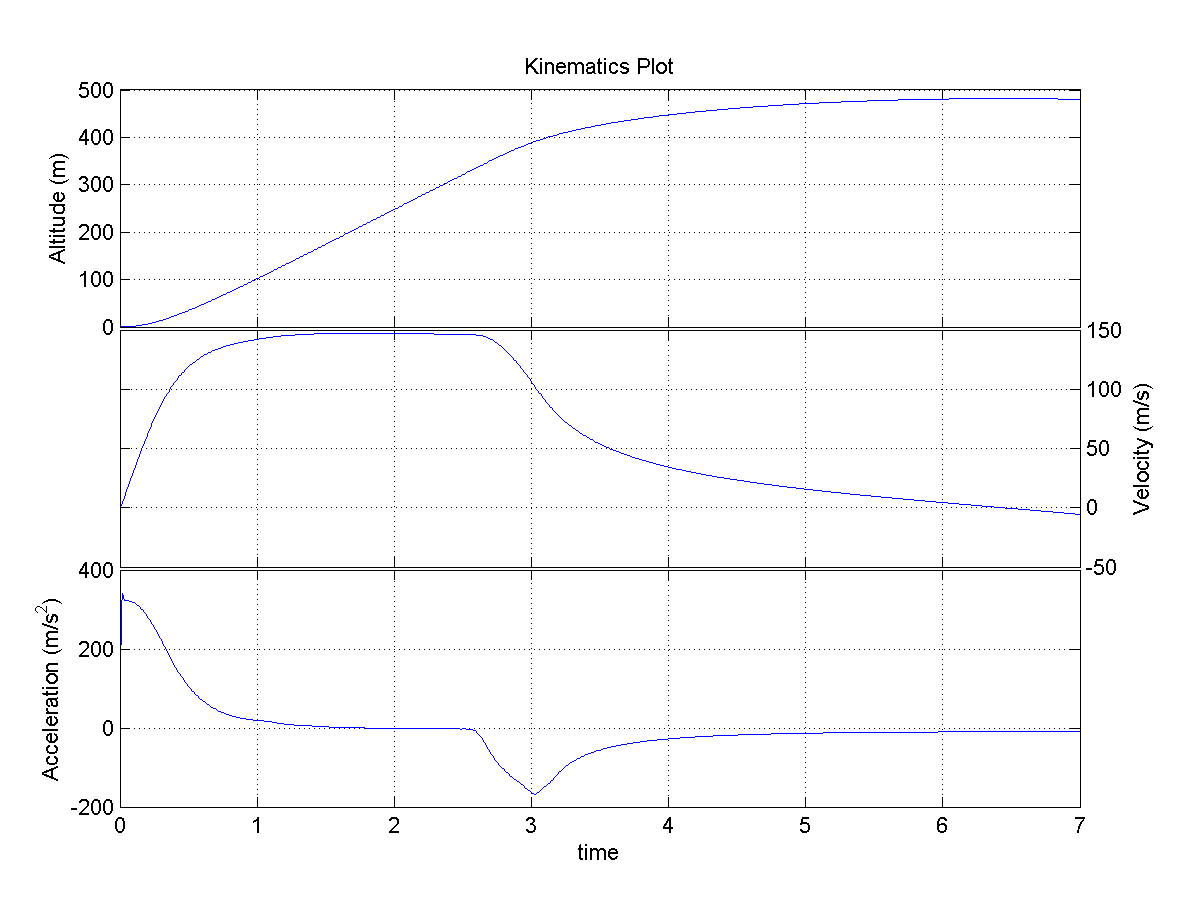
\includegraphics{images/plots/kinematics_plot.png}
\caption{Altitude, Velocity, and Acceleration as a Function of Time
\label{kinematics_plot_label}}
\end{figure}

\begin{figure}[htbp]
\centering
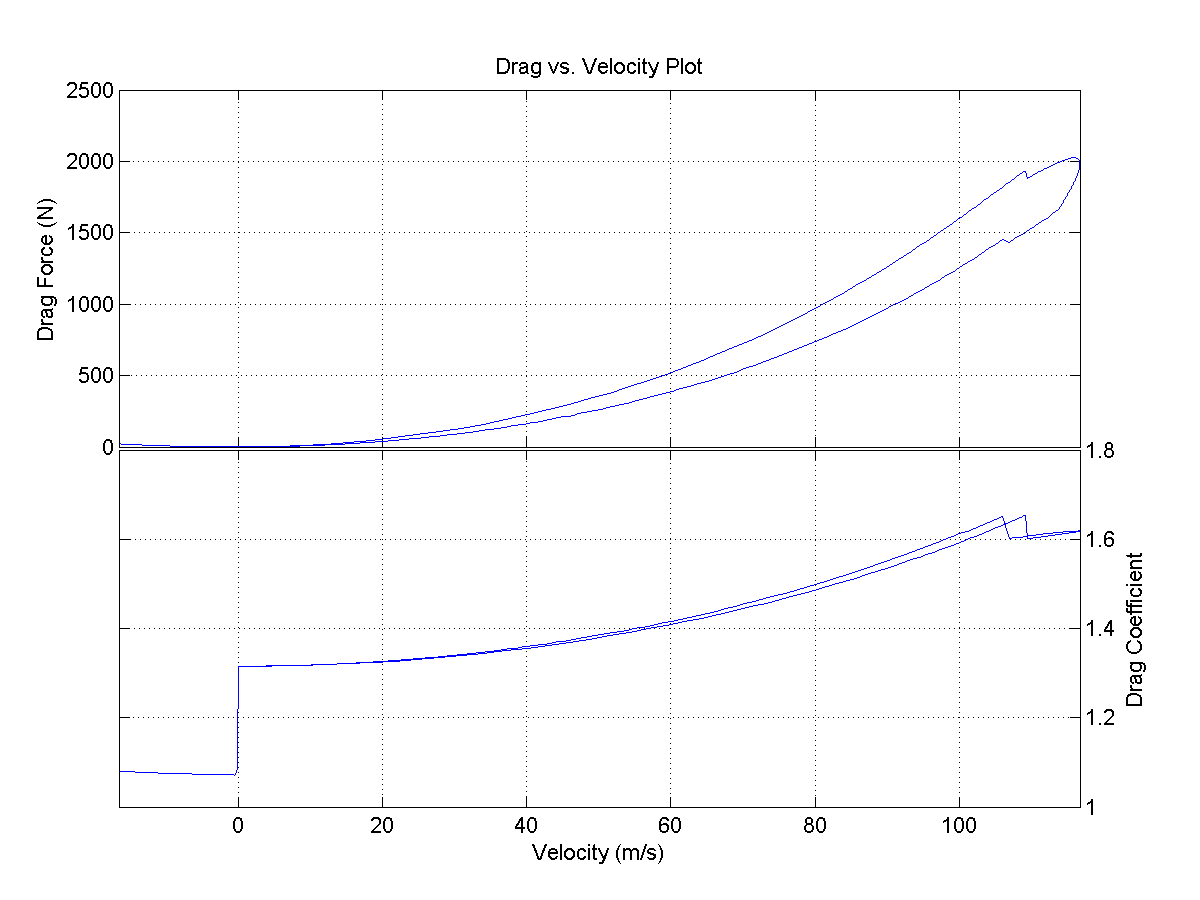
\includegraphics{images/plots/drag_v_velocity_plot.png}
\caption{Drag Force, Drag Coefficient, and Reynolds Number as a Function
of Velocity \label{drag_v_velocity_plot_label}}
\end{figure}

\begin{figure}[htbp]
\centering
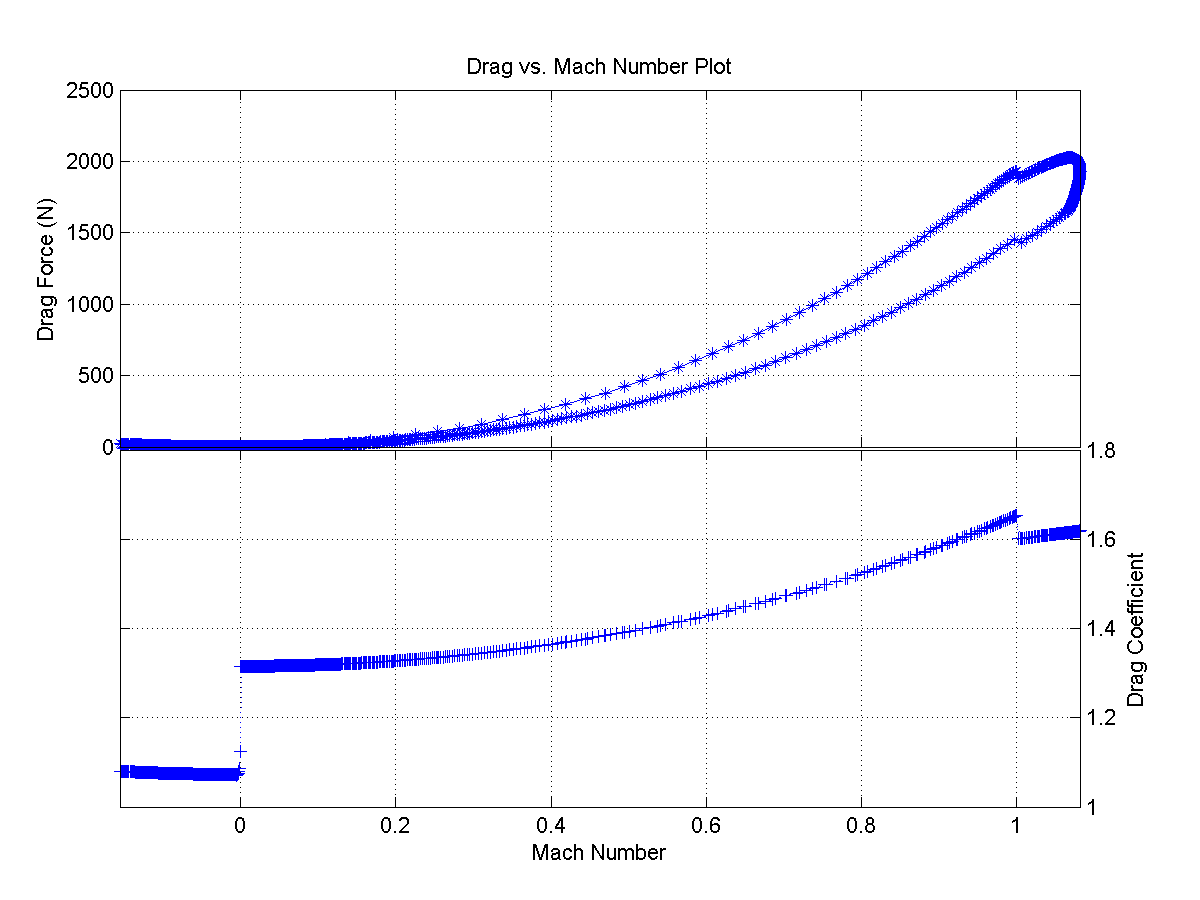
\includegraphics{images/plots/drag_v_mach.png}
\caption{Drag Force, Drag Coefficient, and Reynolds Number as a Function
of Mach Number \label{drag_v_mach_plot_label}}
\end{figure}

\begin{figure}[htbp]
\centering
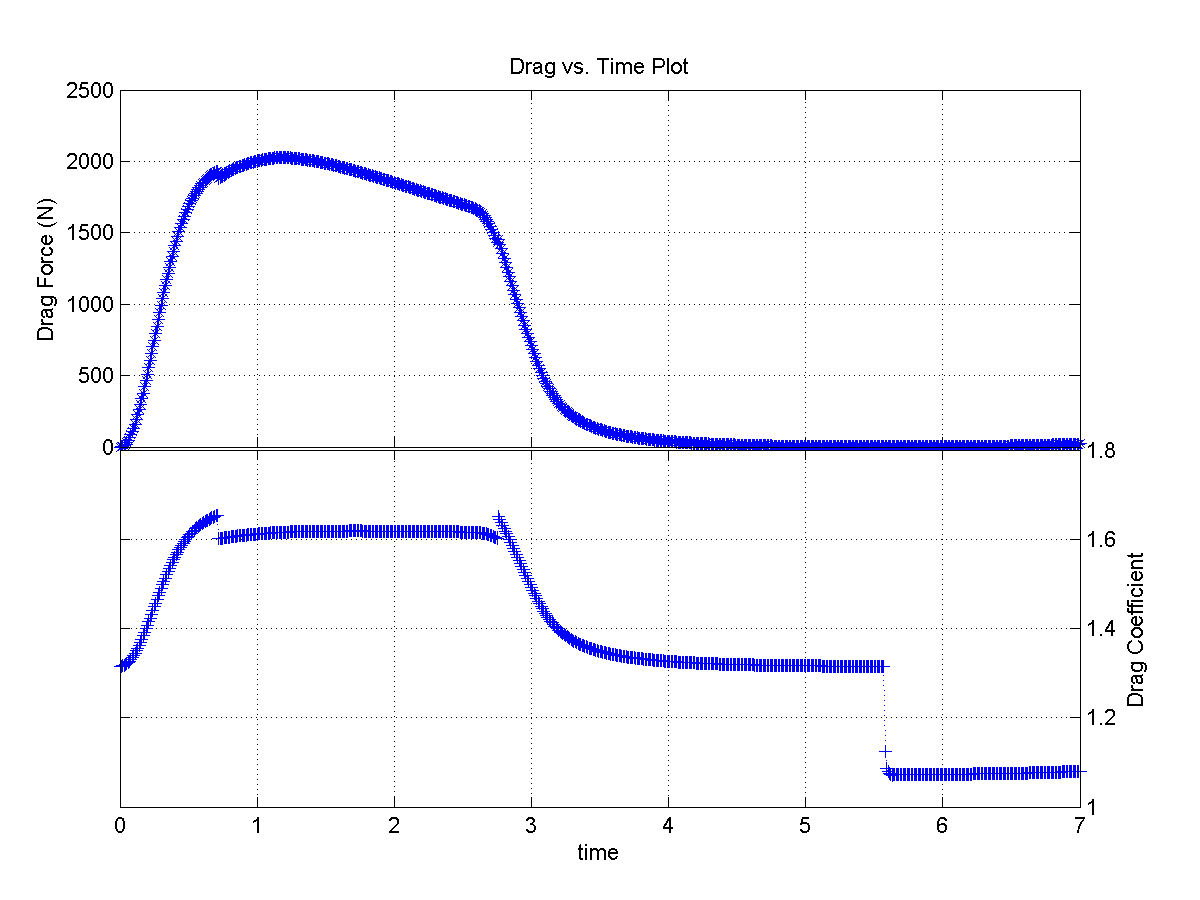
\includegraphics{images/plots/drag_plot.png}
\caption{Altitude, Velocity, and Acceleration as a Function of Time
\label{drag_plot_label}}
\end{figure}

\begin{figure}[htbp]
\centering
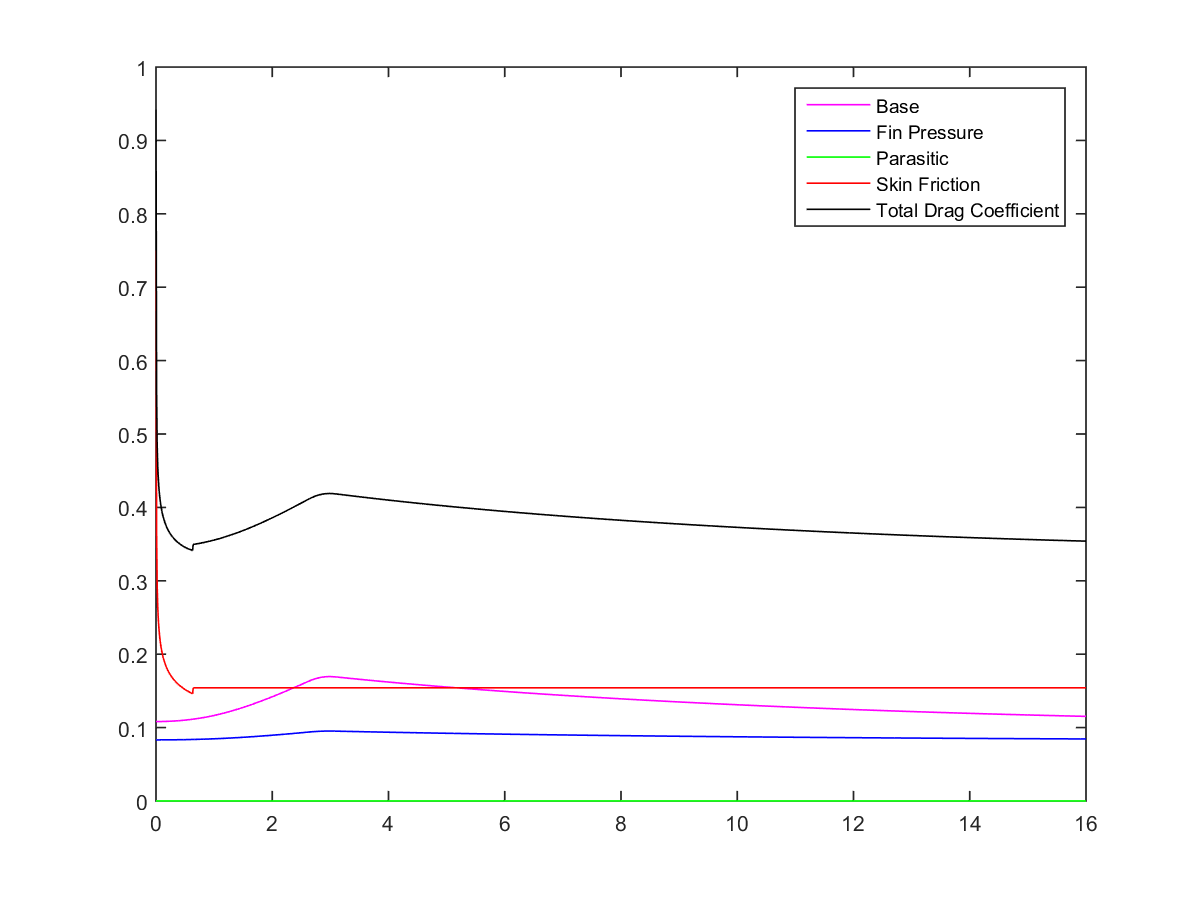
\includegraphics{images/plots/drag_coefficients.png}
\caption{Specific Drag Coefficients as a Function of Time
\label{drag_coefs_plot_label}}
\end{figure}

\begin{figure}[htbp]
\centering
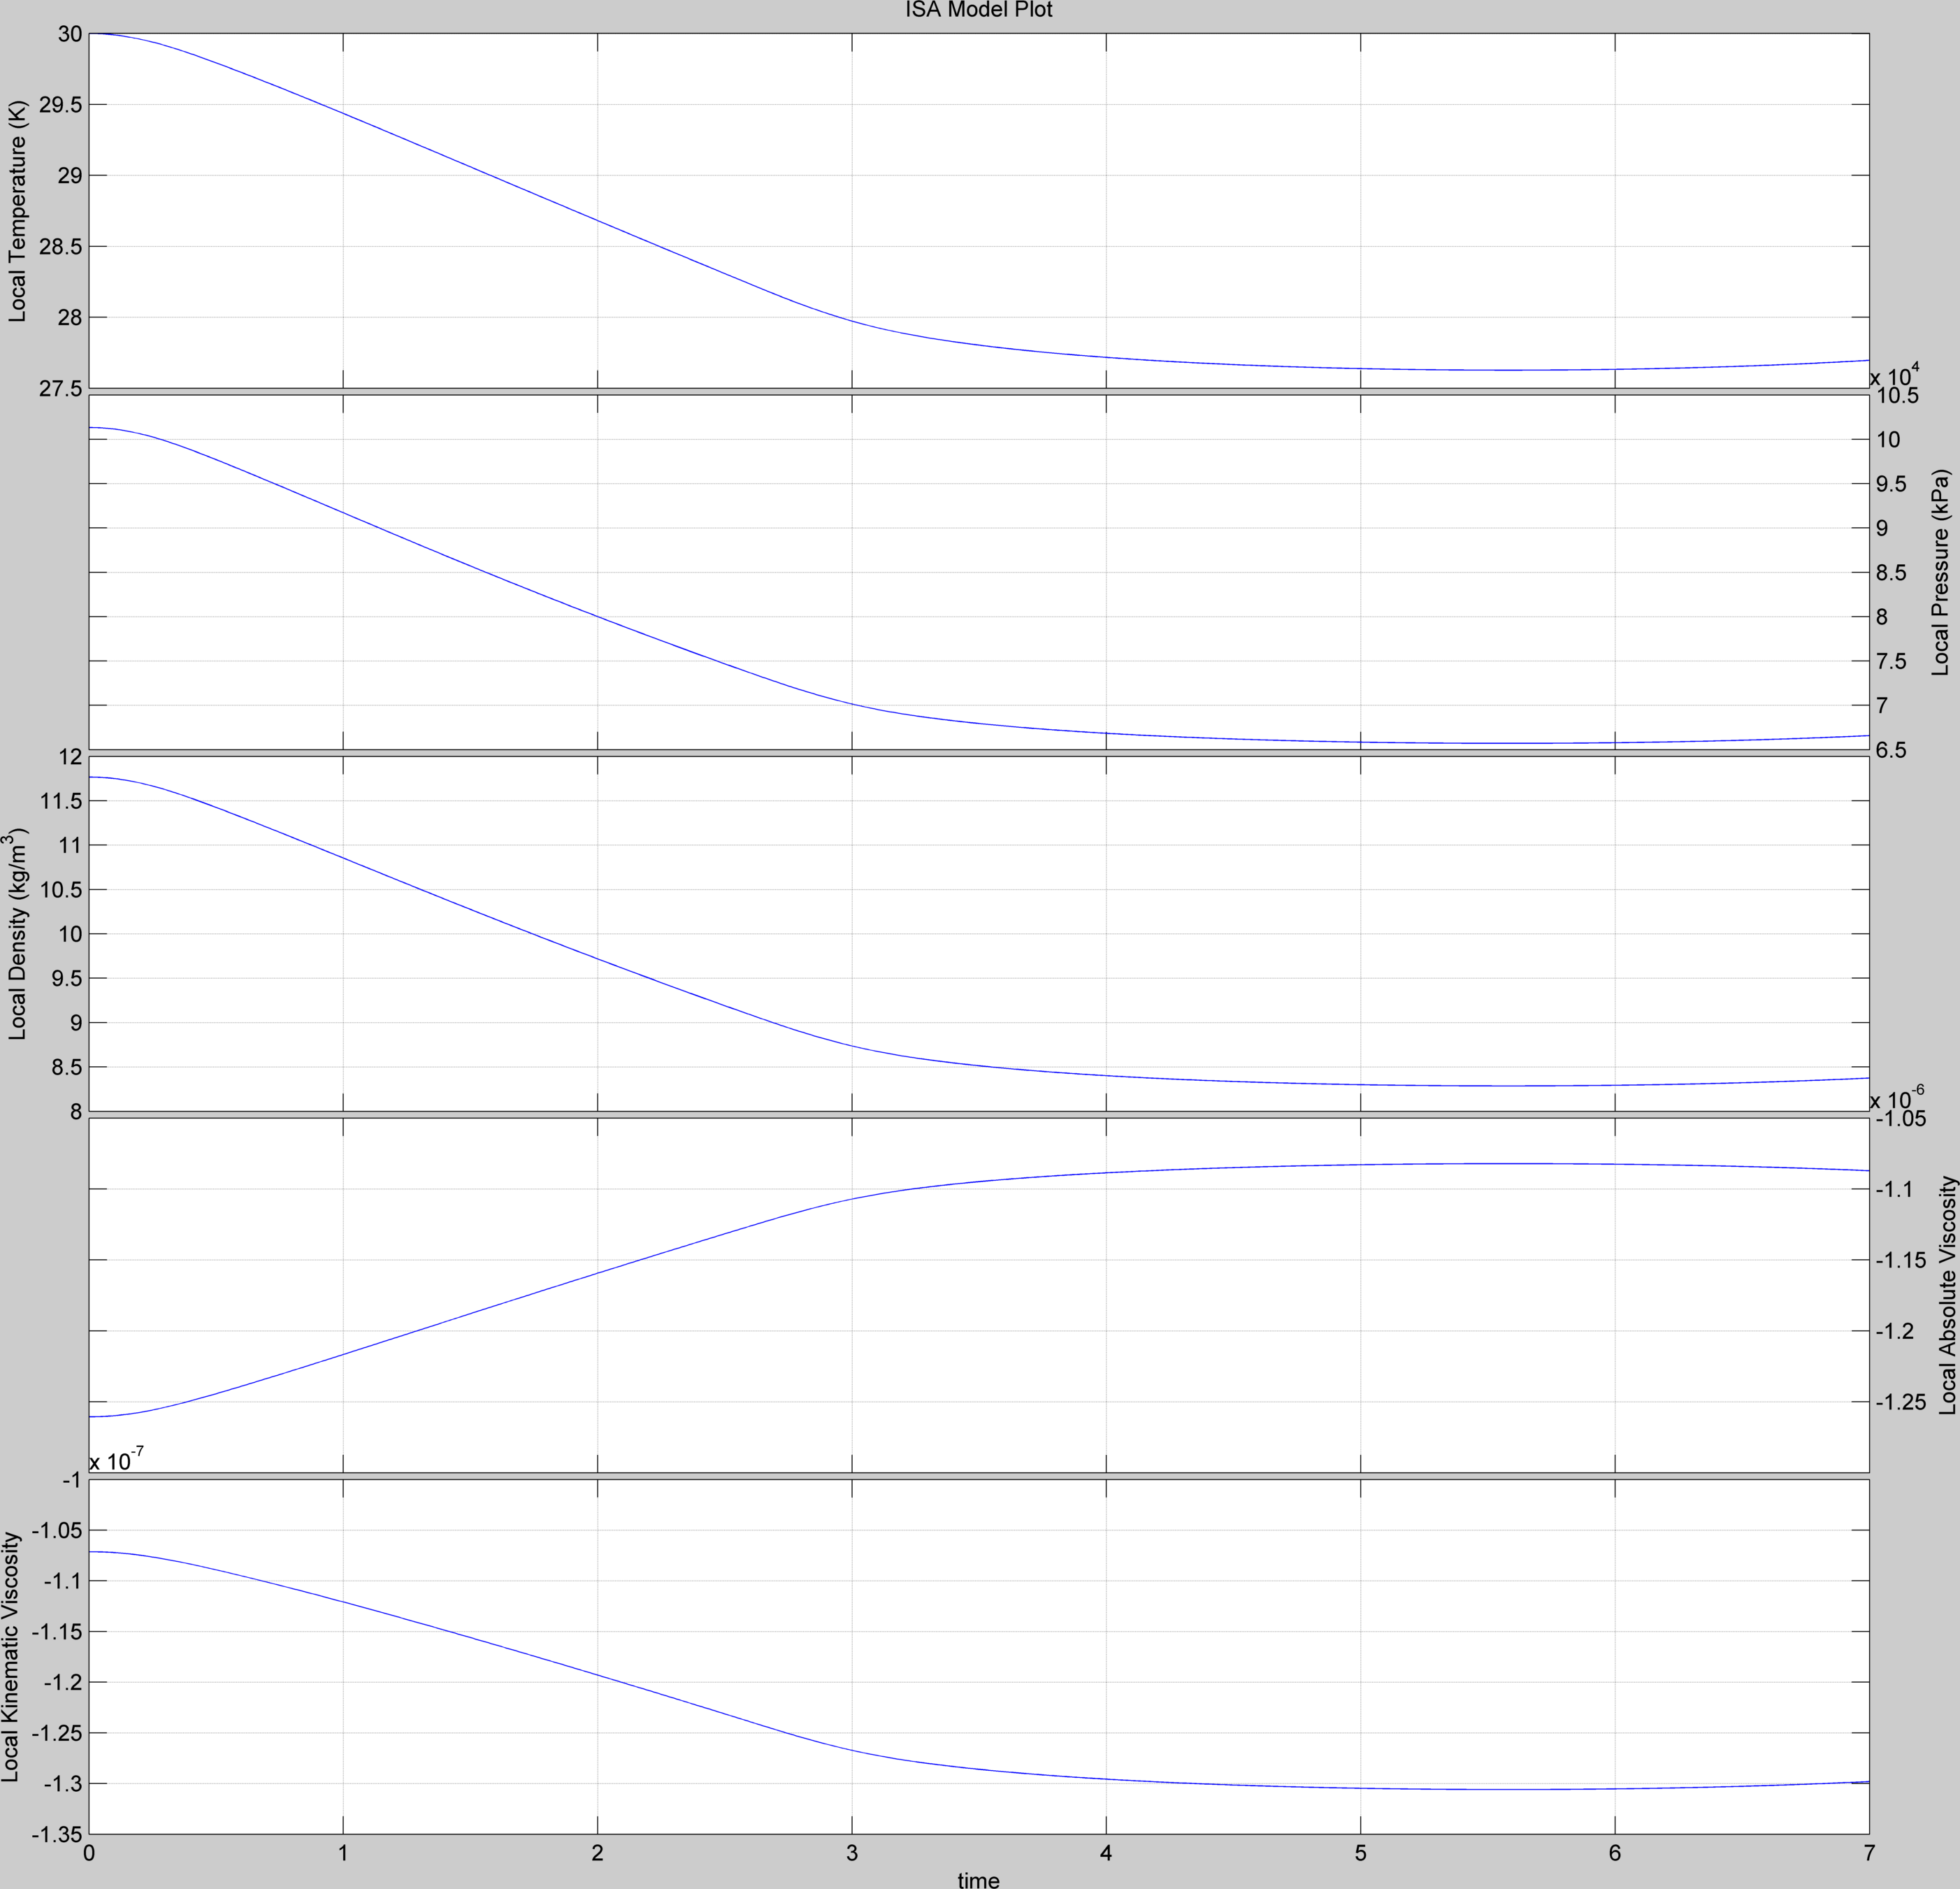
\includegraphics{images/plots/atmosphere_plot.png}
\caption{Altitude, Velocity, and Acceleration as a Function of Time
\label{atmosphere_plot_label}}
\end{figure}

\clearpage

\hyperdef{}{refs}{\label{refs}}
\hyperdef{}{ref-forecastio}{\label{ref-forecastio}}
{[}1{]} F. IO, ``Time machine.'' Online.

\end{document}
